\documentclass[12pt,a4paper]{article}
\usepackage[utf8]{vietnam}
\usepackage{amsmath,amssymb}
\usepackage{geometry}
\geometry{top=1.3cm,bottom=1.2cm,left=1.4cm,right=1.4cm,headheight=15pt,headsep=12pt,footskip=18pt}
\usepackage{tikz}
\usepackage{xcolor}
\usepackage{enumerate}
\usepackage{graphicx}
\usepackage[version=4]{mhchem}
\usepackage{fancyhdr}
\usepackage{ex_test}


\renewcommand{\baselinestretch}{0.95}
\setlength{\parskip}{0pt}

\definecolor{hfRed}{RGB}{211,47,47}
\definecolor{hfGreen}{RGB}{139,195,144}

\pagestyle{fancy}
\fancyhf{}
\fancyhead[L]{\small\itshape\color{hfRed} Tài liệu lưu hành nội bộ}
\fancyhead[R]{\small\itshape\color{hfRed} Thầy \textbf{TRẦN VĂN THẠNH} - 0777.470.803}
\renewcommand{\headrulewidth}{0.8pt}
\renewcommand{\headrule}{\hbox to\headwidth{\color{hfGreen}\leaders\hrule height \headrulewidth\hfill}}

\fancyfoot[L]{\small\itshape\color{hfRed} CS1: 6/15 Nguyễn Hoàng, P. Kim Long, TP Huế \quad|\quad CS2: 24 Đặng Thái Thân, TP Huế}
\fancyfoot[R]{\small\bfseries\color{hfRed} Trang \thepage}
\renewcommand{\footrulewidth}{0.8pt}
\renewcommand{\footrule}{\hbox to\headwidth{\color{hfGreen}\leaders\hrule height \footrulewidth\hfill}}

\fancypagestyle{firstpage}{
  \fancyhf{}
  \renewcommand{\headrulewidth}{0pt}
  \fancyfoot[L]{\small\itshape\color{hfRed} CS1: 6/15 Nguyễn Hoàng, P. Kim Long, TP Huế \quad|\quad CS2: 24 Đặng Thái Thân, TP Huế}
  \fancyfoot[R]{\small\bfseries\color{hfRed} Trang \thepage}
  \renewcommand{\footrulewidth}{0.8pt}
  \renewcommand{\footrule}{\hbox to\headwidth{\color{hfGreen}\leaders\hrule height \footrulewidth\hfill}}
}

\begin{document}
\thispagestyle{firstpage}

\noindent
\begin{minipage}[t]{0.40\textwidth}
	\centering\fontsize{9.5pt}{12pt}\selectfont
	\textbf{SỞ GD\&ĐT THỪA THIÊN HUẾ}\\
	\textbf{TRƯỜNG THPT CAO THẮNG}\\
	\textbf{Mã đề thi: 103}
\end{minipage}\hfill
\begin{minipage}[t]{0.58\textwidth}
	\centering\small
	\textbf{ĐỀ KIỂM TRA CUỐI KÌ II, NĂM HỌC 2023--2024}\\
	\textbf{MÔN: HÓA HỌC 10}\\
	\textit{Thời gian làm bài: 45 phút (không kể thời gian giao đề)}\\
	\textit{(28 câu trắc nghiệm và 03 câu tự luận)}
\end{minipage}

\smallskip
\noindent
Họ và tên: \dotfill Số báo danh: \makebox[4cm]{\dotfill}

\smallskip
\noindent
\textit{Cho biết Nguyên tử khối của: $\ce{Na}=23$; $\ce{K}=39$; $\ce{Al}=27$; $\ce{Br}=80$; $\ce{Cl}=35{,}5$; $\ce{I}=127$; $\ce{O}=16$; $\ce{H}=1$.}

\smallskip
\noindent
\textbf{A. PHẦN TRẮC NGHIỆM (28 CÂU, 07 ĐIỂM).}

\Opensolutionfile{ans}[ans-hs]

\begin{ex}
Enthalpy tạo thành của một chất là
\choice
{nhiệt kèm theo phản ứng trong điều kiện chuẩn}
{nhiệt kèm theo phản ứng tạo thành 1 mol chất đó từ các đơn chất bền nhất}
{nhiệt kèm theo phản ứng tạo thành 1 mol chất đó từ các hợp chất bền nhất}
{nhiệt kèm theo phản ứng trong quá trình đẳng áp}
\end{ex}

\begin{ex}
Tiến hành các thí nghiệm sau:
\begin{enumerate}[(a)]
	\item Cho một mẩu đá vôi ($\ce{CaCO3}$) vào dung dịch $\ce{HCl}$.
	\item Cho $\ce{KBr}$ tác dụng với dung dịch $\ce{H2SO4}$ đặc nóng.
	\item Cho dung dịch $\ce{AgNO3}$ vào dung dịch $\ce{HI}$.
	\item Cho dung dịch $\ce{AgNO3}$ vào dung dịch $\ce{HF}$.
\end{enumerate}
Sau khi kết thúc thí nghiệm, số phản ứng xảy ra thuộc loại phản ứng oxi hóa -- khử là
\choice
{2}
{4}
{3}
{1}
\end{ex}

\begin{ex}
Cho 6 gam $\ce{Zn}$ hạt vào một cốc đựng dung dịch $\ce{H2SO4}$ 4M (dư) ở nhiệt độ thường. Nếu giữ nguyên các điều kiện khác, chỉ biến đổi một trong các điều kiện sau đây:
\begin{enumerate}[(1)]
	\item Thay 6 gam $\ce{Zn}$ hạt bằng 6 gam $\ce{Zn}$ bột.
	\item Thay dung dịch $\ce{H2SO4}$ 4 M bằng dung dịch $\ce{H2SO4}$ 2 M.
	\item Thực hiện phản ứng ở nhiệt độ cao hơn (khoảng $50^\circ\text{C}$).
	\item Dùng thể tích dung dịch $\ce{H2SO4}$ 4 M gấp đôi ban đầu.
\end{enumerate}
Những biến đổi nào làm tăng tốc độ phản ứng?
\choice
{(1), (3)}
{(1), (3), (4)}
{(2), (3), (4)}
{(1), (2), (3), (4)}
\end{ex}

\begin{ex}
Dẫn 2,479 lít (đkc) khí chlorine vào 200 ml dung dịch sodium hydroxide 1,5M ở nhiệt độ thường. Biết phản ứng xảy ra hoàn toàn, khối lượng chất tan có trong dung dịch sau phản ứng là
\choice
{7,45 gam}
{13,30 gam}
{17,30 gam}
{5,85 gam}
\end{ex}

\begin{ex}
Có phản ứng: $\ce{CH4(g) + 2O2(g) ->[t^\circ] CO2(g) + 2H2O(g)}$\\
Cho biết giá trị năng lượng liên kết của một số liên kết:
\begin{center}
\begin{tabular}{|l|c|c|c|c|}
\hline
Liên kết & C--H & O--H & C=O & O=O \\ \hline
$E_b$ (kJ/mol) & 413 & 467 & 745 & 498 \\ \hline
\end{tabular}
\end{center}
Biến thiên enthalpy chuẩn của phản ứng trên là
\choice
{$-710\text{ kJ}$}
{$+668\text{ kJ}$}
{$-978\text{ kJ}$}
{$-434\text{ kJ}$}
\end{ex}

\begin{ex}
Phản ứng nào dưới đây chứng minh tính khử của các ion halide?
\choice
{$\ce{2HCl + CuO -> CuCl2 + H2O}$}
{$\ce{BaCl2 + H2SO4 -> BaSO4 + 2HCl}$}
{$\ce{2HBr + H2SO4 -> Br2 + SO2 + 2H2O}$}
{$\ce{HI + NaOH -> NaI + H2O}$}
\end{ex}

\begin{ex}
Hydrogen halide có nhiệt độ sôi cao nhất là
\choice
{$\ce{HCl}$}
{$\ce{HI}$}
{$\ce{HBr}$}
{$\ce{HF}$}
\end{ex}

\begin{ex}
Nhận định nào sau đây đúng?
\choice
{Bất cứ phản ứng nào cũng cần tăng áp suất để tăng tốc độ phản ứng}
{Chất xúc tác là chất làm tăng tốc độ phản ứng và biến mất sau khi phản ứng kết thúc}
{Chất xúc tác làm tăng tốc độ phản ứng nhưng vẫn được bảo toàn về chất và lượng khi kết thúc phản ứng}
{Bất cứ phản ứng nào cũng cần chất xúc tác để tăng tốc độ phản ứng}
\end{ex}

\begin{ex}
Dựa vào phương trình nhiệt hóa học của phản ứng:
\[\ce{CO2(g) -> CO(g) + 1/2 O2(g)} \quad \Delta_r H^\circ_{298} = +280\text{ kJ}\]
Giá trị $\Delta_r H^\circ_{298}$ của phản ứng: $\ce{2CO2(g) -> 2CO(g) + O2(g)}$ là
\choice
{$+560\text{ kJ}$}
{$-420\text{ kJ}$}
{$+140\text{ kJ}$}
{$-1120\text{ kJ}$}
\end{ex}

\begin{ex}
Trong tự nhiên, các halogen
\choice
{tồn tại ở cả dạng đơn chất và hợp chất}
{chỉ tồn tại ở dạng muối halide}
{chỉ tồn tại ở dạng đơn chất}
{chỉ tồn tại ở dạng hợp chất}
\end{ex}

\begin{ex}
Phát biểu \textbf{không} chính xác là
\choice
{Trong tất cả các hợp chất, fluorine chỉ có số oxi hóa -1}
{Trong tất cả các hợp chất, các halogen chỉ có số oxi hóa là -1}
{Trong hợp chất với hydrogen và kim loại, các halogen luôn thể hiện số oxi hóa là -1}
{Tính oxi hóa của halogen giảm dần từ fluorine đến iodine}
\end{ex}

\begin{ex}
Ý nghĩa của hệ số nhiệt độ Van't Hoff ($\gamma$) là
\choice
{giá trị của $\gamma$ càng lớn thì ảnh hưởng của nhiệt độ đến tốc độ phản ứng càng mạnh}
{giá trị của $\gamma$ càng lớn thì tốc độ phản ứng càng giảm}
{giá trị của $\gamma$ càng lớn thì ảnh hưởng của nhiệt độ đến tốc độ phản ứng càng yếu}
{giá trị của $\gamma$ càng lớn thì tốc độ phản ứng càng tăng}
\end{ex}

\begin{ex}
Dung dịch dùng để nhận biết các ion halide là
\choice
{$\ce{NaOH}$}
{quỳ tím}
{$\ce{HCl}$}
{$\ce{AgNO3}$}
\end{ex}

\begin{ex}
Trong các phản ứng hoá học, để chuyển thành anion, nguyên tử của các nguyên tố halogen đã nhận hay nhường bao nhiêu electron?
\choice
{Nhường đi 1 electron}
{Nhận thêm 1 electron}
{Nhận thêm 2 electron}
{Nhường đi 7 electron}
\end{ex}

\begin{ex}
Chuẩn bị 3 ống nghiệm, các dung dịch có cùng nồng độ 0,1M. Tiến hành thí nghiệm theo các bước:
\begin{itemize}
	\item Bước 1: Cho vào mỗi ống nghiệm khoảng 2 mL dung dịch các chất như hình vẽ:
\end{itemize}
\begin{center}
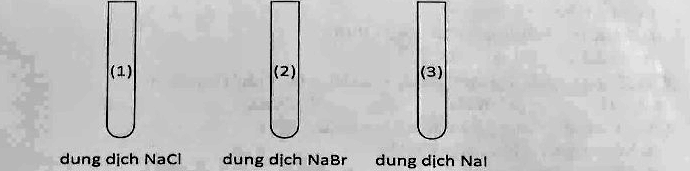
\includegraphics[width=6.5cm]{images_crop/fig_cau15_ongnghiem.png}
\end{center}
\begin{itemize}
	\item Bước 2: Cho vào mỗi ống nghiệm khoảng 1 mL nước chlorine.
	\item Bước 3: Thêm tiếp vào mỗi ống nghiệm vài giọt dung dịch $\ce{AgNO3}$.
\end{itemize}
Cho các phát biểu sau:
\begin{enumerate}[(1)]
	\item Cả ba ống nghiệm đều xuất hiện kết tủa trắng ở bước 2.
	\item Sau bước 3, chỉ có ống nghiệm (1) thu được kết tủa trắng.
	\item Từ hiện tượng quan sát được có thể kết luận tính oxi hoá của chlorine mạnh hơn của bromine và iodine.
	\item Dung dịch ở ống (1) không thể phản ứng với nước bromine.
\end{enumerate}
Số phát biểu đúng là
\choice
{2}
{3}
{1}
{4}
\end{ex}

\begin{ex}
Cho các biến đổi sau:
\begin{enumerate}[(1)]
	\item Đun nóng chất tham gia.
	\item Thêm chất xúc tác phù hợp.
	\item Pha loãng dung dịch.
	\item Giảm nhiệt độ.
	\item Tăng nhiệt độ.
	\item Giảm diện tích bề mặt tiếp xúc.
	\item Tăng nồng độ chất phản ứng.
	\item Chia nhỏ chất phản ứng thành nhiều mảnh nhỏ.
\end{enumerate}
Có bao nhiêu biến đổi làm tăng tốc độ phản ứng?
\choice
{5}
{7}
{6}
{4}
\end{ex}

\begin{ex}
Cấu hình electron lớp ngoài cùng của nguyên tử các nguyên tố halogen là
\choice
{$ns^2np^6$}
{$ns^2np^4$}
{$ns^2np^5$}
{$ns^2np^3$}
\end{ex}

\begin{ex}
Trong phản ứng: $\ce{3Cu + 8HNO3 -> 3Cu(NO3)2 + 2NO + 4H2O}$. Số phân tử nitric acid ($\ce{HNO3}$) đóng vai trò chất oxi hóa là
\choice
{4}
{2}
{8}
{6}
\end{ex}

\begin{ex}
Loại liên kết yếu được hình thành giữa nguyên tử H (đã liên kết với một nguyên tử có độ âm điện lớn, thường là F, O, N) với một nguyên tử khác (có độ âm điện lớn, thường là F, O, N) còn cặp electron hóa trị chưa tham gia liên kết là
\choice
{liên kết cộng hóa trị có cực}
{liên kết hydrogen}
{liên kết ion}
{liên kết cộng hóa trị không cực}
\end{ex}

\begin{ex}
Tốc độ của một phản ứng có dạng: $v = k \cdot C_A^x \cdot C_B^y$ (A, B là 2 chất khác nhau). Nếu tăng nồng độ chất A lên 2 lần, nồng độ chất B không đổi thì tốc độ phản ứng tăng 8 lần. Giá trị của x là
\choice
{6}
{3}
{8}
{4}
\end{ex}

\begin{ex}
Yếu tố áp suất ảnh hưởng đến tốc độ phản ứng nào dưới đây?
\choice
{$\ce{2CO(g) + O2(g) -> 2CO2(g)}$}
{$\ce{Fe(s) + S(s) -> FeS(s)}$}
{$\ce{NaOH(aq) + HCl(aq) -> NaCl(aq) + H2O(l)}$}
{$\ce{NH4Cl(s) -> NH3(g) + HCl(g)}$}
\end{ex}

\begin{ex}
Trong phản ứng $\ce{Zn + CuSO4 -> ZnSO4 + Cu}$. Chất bị oxi hóa là
\choice
{$\ce{CuSO4}$}
{$\ce{Zn}$}
{$\ce{ZnSO4}$}
{$\ce{Cu}$}
\end{ex}

\begin{ex}
Đặc điểm chung của đơn chất halogen là
\choice
{Vừa có tính oxi hóa vừa có tính khử}
{Có tính oxi hóa mạnh}
{Tác dụng mạnh với nước}
{Ở điều kiện thường là chất khí}
\end{ex}

\begin{ex}
Cho phương trình hóa học của phản ứng: $\ce{2A + B -> C}$. Biểu thức tính tốc độ tức thời của phản ứng là
\choice
{$v = k \cdot C_A \cdot C_B$}
{$v = k \cdot C_A^2 \cdot C_B$}
{$v = 2k \cdot C_A^2 \cdot C_B$}
{$v = k \cdot C_A \cdot C_B^2$}
\end{ex}

\begin{ex}
Cho các phát biểu sau:
\begin{enumerate}[(1)]
	\item Nước Javel có khả năng tẩy màu và sát khuẩn.
	\item Cho $\ce{Cl2}$ vào dung dịch $\ce{NaOH}$ đun nóng ta thu được nước Javel.
	\item Hydrofluoric acid là acid yếu.
	\item Tính khử của các ion halide tăng dần theo thứ tự: $\ce{F-}$, $\ce{Cl-}$, $\ce{Br-}$, $\ce{I-}$.
	\item Khí chlorine ẩm và nước chlorine đều có tính tẩy màu.
\end{enumerate}
Trong các phát biểu trên, số phát biểu đúng là
\choice
{1}
{3}
{4}
{2}
\end{ex}

\begin{ex}
Cho phương trình nhiệt hoá học:
\[\ce{2Al_{(s)} + Fe2O3_{(s)} -> Al2O3_{(s)} + 2Fe_{(s)}} \quad \Delta_r H^\circ_{298} = -851{,}5\text{ kJ}\]
Phản ứng này là phản ứng
\choice
{tỏa nhiệt}
{trao đổi}
{trung hòa}
{thu nhiệt}
\end{ex}

\begin{ex}
Trong phản ứng hoá học, tốc độ phản ứng
\choice
{tỉ lệ nghịch với nhiệt độ của phản ứng}
{tăng khi nhiệt độ của phản ứng tăng}
{giảm khi nhiệt độ của phản ứng tăng}
{không đổi khi nhiệt độ của phản ứng tăng}
\end{ex}

\begin{ex}
“Bảo quản thức ăn trong tủ lạnh để thức ăn lâu bị ôi thiu”. Yếu tố nào đã ảnh hưởng đến tốc độ phản ứng trong tình huống thực tiễn trên?
\choice
{Diện tích bề mặt}
{Nhiệt độ}
{Chất xúc tác}
{Nồng độ}
\end{ex}

\Closesolutionfile{ans}

\vspace{0.3cm}
\noindent
\textbf{B. PHẦN TỰ LUẬN (03 CÂU, 03 ĐIỂM).}

\begin{ex}
Hoàn thành phương trình hóa học của các phản ứng sau:
\begin{enumerate}[a.]
	\item $\ce{Br2} + \dots \rightarrow \ce{KBr} + \ce{I2}$
	\item $\ce{KMnO4} + \dots \rightarrow \dots + \dots + \ce{Cl2} + \ce{H2O}$
	\item $\ce{Fe + Cl2 ->[t^\circ]} \dots$
	\item $\ce{Cl2 + NaOH ->[t^\circ] NaCl} + \dots + \ce{H2O}$
\end{enumerate}
\loigiai{}
\end{ex}

\begin{ex}
Để hoà tan hết một mẫu $\ce{Al}$ trong dung dịch $\ce{HCl}$ ở $25^\circ\text{C}$ cần 36 phút. Cũng mẫu $\ce{Al}$ đó tan hết trong dung dịch acid nói trên ở $45^\circ\text{C}$ trong 4 phút. Hỏi để hoà tan hết mẫu $\ce{Al}$ đó trong dung dịch acid nói trên ở $60^\circ\text{C}$ thì cần thời gian bao nhiêu giây?
\loigiai{}
\end{ex}

\begin{ex}
Theo tính toán của các nhà khoa học, để phòng bệnh bướu cổ và một số bệnh khác, mỗi người cần bổ sung $1{,}5 \cdot 10^{-4}\text{ g}$ nguyên tố iodine mỗi ngày. Nếu lượng iodine đó chỉ được bổ sung từ muối iodised (còn gọi là muối iot, chứa 25g $\ce{KI}$ trong một tấn muối) thì mỗi người cần bao nhiêu gam muối mỗi ngày?
\loigiai{}
\end{ex}

\begin{center}
\textbf{---------HẾT---------}
\end{center}

\end{document}
